In the following steps, you will create a \gdcase{} which  contains four \gdcases{} to enter values into the two fields in the Adder program, click the equals button and check the result. In doing this, you will learn to use a feature of \app{} that lets you execute actions on different components. You will also learn how to add data from Excel tables. 

\begin{enumerate}
\item In the \gdtestcasebrowser{} right-click and select:\\ \bxmenu{New}{\gdcase{}}{}. 
\item In the dialog which appears, name the \gdcase{}: \bxname{TestAdder}.
 \item Click \bxcaption{OK}. 
 \item You will see the \gdcase{} you just created as a node in the \gdtestcasebrowser{} (\bxfigref{TutCaseInBrowser}).
\item Double-click on this node to open the \gdtestcaseeditor{}. 
\item In this editor, right-click and select:\\ \bxmenu{Add}{Existing \gdcase{}}{}.
\item You will see a dialog which offers you all the \gdcases{} you can reference at this point (\bxfigref{TutAddExistingTestCase}).

\begin{figure}[h]
\begin{center}
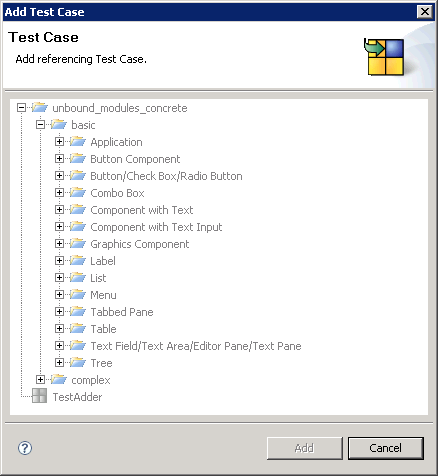
\includegraphics{Tutorials/PS/TutAddExistingTestCase}
\caption{Adding an existing \gdcase{}}
\label{TutAddExistingTestCase}
\end{center}
\end{figure}

\item Navigate to the category:\\ \bxname{Basic/Component With Text Input/Replace Text}\\ and select the \gdcase{}:\\
\bxname{ub\_cti\_replaceText}.
\bxtipp{We are using \bxname{component with text input} instead of \bxname{textfield} because we can map abstract components like \bxname{component with text input} to more real components in the \gdaut{}. This makes the \gdcase{} more reusable because it is more generic.}
\item Click \bxcaption{Add}.
\item The \gdcase{} you selected appears in the \gdtestcaseeditor{}.

\bxtipp{The \gdcases{} are named according to conventions \bxpref{BPComponentNames}. The name is composed of an \gdaut{} name (if the \gdcase{} is \gdaut{}-specific -- in this case, \bxname{ub} means \bxname{unbound}), an abbreviation for the component type, and the action carried out. }
\item Add three more \gdcases{} to the \bxname{TestAdder} \gdcase{} using drag and drop from the \gdcase{} browser. The \gdcases{} you need are:\\
\begin{itemize}
\item In the category \bxname{Basic/Component With Text Input/Replace Text}, the \gdcase{ub\_cti\_replaceText} (again).
\item  In the category \bxname{Basic/Button Component/Click}, the \gdcase{ub\_btc\_click}.
\item  In the category \bxname{Basic/Component with Text}, the \gdcase{ub\_ctx\_checkText\_equals}.
\end{itemize}

Your \gdtestcaseeditor{} should now contain four \gdcases{} (\bxfigref{TutTCEditor}). 

\begin{figure}[h]
\begin{center}
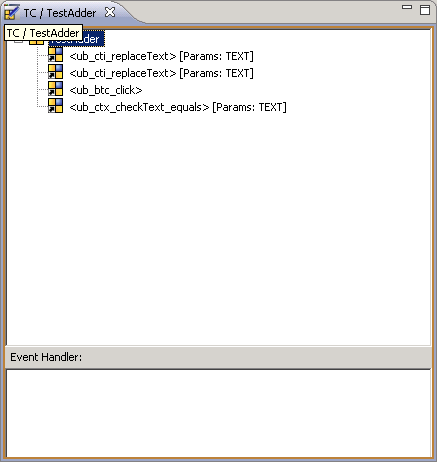
\includegraphics{Tutorials/PS/TutTCEditor}
\caption{The TestAdder \gdcase{}}
\label{TutTCEditor}
\end{center}
\end{figure}

\item In the first \gdcase{}, enter a reference for the parameter in the \bxname{Parameter} field in the \gdpropview{}, e.g. \bxshell{=VALUE1}. Then press \bxkey{enter}. The referenced parameter appears next to the top \gdcase{} in the \gdtestcaseeditor{}.

Click on the \gdcompnamesview{} and enter a new name for the component, e.g. \bxshell{Adder\_value1\_textfield}. The original name (\bxname{nn\_nn\_cti}) is a placeholder for more meaningful component names when the \gdcase{} is reused. Again, the name is made up of three parts: the \gdaut{} it is used in, the GUI-component, and the type of component. In larger applications, you can also add details about which dialog the component is in. 

\item In the second \gdcase{}, enter \bxshell{=VALUE2} in the \bxname{Parameter} field in the \gdpropview{} and press \bxkey{enter}. 

Click on the \gdcompnamesview{} and enter a new name for the component, e.g. \bxshell{Adder\_value2\_textfield}. Even though this \gdcase{} is the same as the first \gdcase{}, we have now specified that it will execute the action on a different component and with different data than the first \gdcase{}. 

\item In the fourth \gdcase{}, enter \bxshell{=RESULT} in the \bxname{Parameter} field in the \gdpropview{} and press \bxkey{enter}. 

Click on the \gdcompnamesview{} and enter a new name for the component, e.g. \bxshell{Adder\_result\_textfield}.
 
\item Now the \bxname{TestAdder} \gdcase{} should have three parameters: VALUE1, VALUE2 and RESULT. 
\end{enumerate}



